
\subsection{Functional requirements}
We assume that all domain properties stipulated in paragraph 1.6 hold. We decided to use a \textit{goal-driven} method to structure our requirements, meaning that we decomposed the high-level goals of paragraph 1.5 into low-level requirements.
Some of these requirements stem directly from the requests of our clients, while others are born from the necessity to have a sound system.

For each goal, we derive the following requirements:



\begin{itemize}


				\item \textit{G[1]} The system allows guests to register; to complete the registration procedure the system sends a password to the guest as an access key.
					\begin{itemize}
						\item R[1.1] The system has to allow any person to submit only one account request.
						\item R[1.2] The system must accept an account requrest only if the credit card owner's name and the user's name coincide.
						\item R[1.3] The account is created when an admin validates all the necessary data.
						\item R[1.4] The system must be able to generate passwords.
						\item R[1.5] The system has to send a newly generated password to the user via email when the account is created.
						\item R[1.6] The system must be able to check whether a password is correct or not.
						\item R[1.7] The system must let the user log in only if the password is correct. 
						\item R[1.8] The system has to generate a new password and send it via email if the user asks for it.
					\end{itemize}

				\item \textit{G[2]} The system should enable a registered user to find the location of an available car within a certain distance from the user's location or from a specified address.
					\begin{itemize}
						\item R[2.1] The system must have the ability to locate the user.
						\item R[2.2] The system must be able to locate any valid address.
						\item R[2.3] The system must be able to find any of the parking areas of the company. 
						\item R[2.4] The system must be able to identify available cars inside parking areas.
						\item R[2.5] The system must let users see whether there are available cars in a specified radius. %XXX
					\end{itemize}
					
				\item \textit{G[3]} The system enables user to reserve a single available car in a certain geographical region for one hour before the user picks it up. If the car is not picked up by that time, the reservation expires, the system tags this car as available again and it charges the user a fine of 1 EUR.
					\begin{itemize}
						\item R[3.1] The system must allow users to reserve an available car.
						\item R[3.2] The cars cannot be reserved by more than one user at any given time.
						\item R[3.3] The system must keep the current reservation standing until the user has opened the car or an hour has passed. %FIXME "An hour" -> a predefined time?? This is a parameter!!!
						\item R[3.4] The system must be able to autonomously cancel reservations.
						
						\item R[3.5] The system must impede any user with an expired license to reserve a car.
						\item R[3.6] The system must impede any banned user to reserve a car.
						%TODO others?
					\end{itemize}

				\item \textit{G[4]} The system should allow the user to employ a car in a proper and safe way. 
					\begin{itemize}
						\item R[4.1] The system must be able to locate any car at any given time. 
						\item R[4.2] The system must be able to detect whether there are passengers inside a car, and how many.
						\item R[4.3] The system must be able to collect data about the power charge of any of its cars.
						\item R[4.4] The system must be able to detect when a severe accident has occurred to a car.
						\item R[4.5] The system must be able to detect when a user is near a car.
						\item R[4.6] The system must be able to tell when a car is parked in a safe area.
						\item R[4.7] The system must be able to detect when a car is plugged to the power grid.
						\item R[4.8] The system must be able to detect whether the driver is still in the car.
						\item R[4.9] The system must be able to automatically unlock a car when the user that has reserved is nearby. %NOTE attention to alloy for inconsistency!!!
						\item R[4.10] The system must be able to automatically lock a car when the user has exited it inside a safe area. 
						\item R[4.11] The system must allow the user to lock and unlock their car manually when outside a safe area.
						\item R[4.12] The system must provide a finite time window that begins when the user exits the car inside a safe area. The time window must either end when the allotted time is finished or when another user reserves the same car.
						\item R[4.13] The system must allow the user to re-enter the car while the time window is still open. 
					\end{itemize}
					
				\item \textit{G[5]} The system charges the user for a predefined amount of money per minute. A screen on the car notifies the user of the current charges.
					\begin{itemize}
						\item R[5.1] The system must be able to retrieve all data necessary to charge the user. This data is the duration of the ride and all the conditions for the eventual application of discounts and sanctions.
						\item R[5.2] The system should notify the user of the fee per minute he's being charged through a screen inside the car.
						\item R[5.3] The system must notify the final charges to the user after the time window for the ride has expired.
						\item R[5.4] The system must invoice the user after the time window for the ride by communicating the charges to the external payment system. 
						
					\end{itemize}
				
				\item \textit{G[6]} The system starts charging the user as soon as the car ignites. It stops charging them when the car is parked in a safe area and the user exits the car.
					\begin{itemize}
						\item R[6.1] The system must charge the user with a fee per minute.
						\item R[6.2] The system must be able to tell when the car has ignited. 
						\item R[6.3] The system should start counting the charges from the ignition onward. %FIXME horridly put
						\item R[6.4] The system must stop counting the charges when the user exits the car while inside a safe area.
						\item R[6.5] If the reservation has expired but the user is inside the car (without igniting it), the system must start charging them anyway an exceptional fee per minute. %cfr requirements for G11
					\end{itemize}
					
				\item \textit{G[7]} The system should encourage good user behaviour through the application of discounts to the fee per minute. 
					\begin{itemize}
						\item R[7.1] The system must apply all discounts to the fee per minute.
						\item R[7.2] If the conditions for a discount are satisfied only for a limited period of time during the ride, the discount should be applied only to that time period. %This basically only happens with the passengers & money saving option if you think abt that.
						\item R[7.3] The system must apply a discount every time a user brings two or more passengers in the car with them.
						\item R[7.4] The system must apply a discount every time the car has more than 50\% of power charge by the end of a standard ride. %FIXME horridly put
						\item R[7.5] The system must be able to apply a discount to a ride every time the car for that ride is plugged to the power grid at the end of the time window. 
					\end{itemize}
					
				\item \textit{G[8]} The system should discourage bad behaviour through the application of sanctions to the fee per minute.
					\begin{itemize}
						\item R[8.1] The system must apply a sanction every time a car is returned in a safe area at more than 3 km from the nearest recharging safe area.
						\item R[8.2] The system must apply a sanction every time a car is returned with less than 20\% of power charge.
					\end{itemize}
					
				\item \textit{G[9]} The system should provide an alternative usage mode for cars called \textit{money saving option}. Besides aiding the user in saving money, this mode allows for a uniform distribution of cars throughout the city by suggesting the user where to park.
					\begin{itemize}
						\item R[9.1] The system must always allow a user to select the \textit{money saving option} at any point during their ride. 
						\item R[9.2] The system must apply a discount every time the car is returned in the suggested safe area with the \textit{money saving} option.
						\item R[9.3] The system must select the safe area suggested to the user based on consideration of availability of power plugs and of distribution of the cars. This safe area must be as close as possible to the user's destination. %FIXME rewrite; too generic
					\end{itemize}
					
				\item \textit{G[10]} The system allows the company to assist the users in case of need and take care of the cars.	
					\begin{itemize}
						\item R[10.1] The system must always allow a user to notify the back-end administrators if they have a problem with the car.
						\item R[10.2] The system must always be able to locate \textit{PowerEnJoy} operators. 
						\item R[10.3] The system must allow administrators to know the status of on-site operators and dispatch them if they are available.
						\item R[10.4] The system must keep track of every car's battery and alert the admin when it lowers below 3\%. 
						\item R[10.5] The system must always notify the admin when it detects that an accident occurred. 
						\item R[10.6] If the system has already notified the admin of an accident, then it must prevent the user from notifying it again.
						\item R[10.7] If the system has already notified the admin of an accident, then it must notify the user of this fact.
					\end{itemize}
					
				\item \textit{G[11]} The admin should be able to configure some parameters of the system.
					\begin{itemize}
						\item R[11.1] The system must allow the aministrators to modify parameters that influence the usage of cars. This parameters are:
							\begin{enumerate}
								\item The standard fee per minute
								\item The exceptional fee per minute
								\item The lost reservation fee
								\item The fine for leaving an accident site %TODO shouldn't we explain our reasoning for accidents/incidents somewhere??
								\item Discount percent values
								\item Sanction percent values
								\item Time window for reservation fee
								\item Time window after ending the ride for reopening and pluggin the car.
							\end{enumerate}
					\end{itemize}
\end{itemize}





\subsection{Non-functional requirements}
	\subsubsection{User interface}
	\paragraph{}The interface of our application is thought to be used mainly via mobile app, with some content also displayed in a web page. The team reasoned that the main functionalities of the system (such as reserving and managing a car) make sense only in a \textit{movable} context (meaning, such that the user can do them anywhere they have an internet connection). Those functionalities are available on the mobile app. On the other hand, operations such as signing up are more easily managed in front of a computer, so the web page allows users to register, login and manage their profiles (which they can do also via mobile app anyway).
	\paragraph{}We pondered on the possibility of adding the possibility of reserving a car via web browser. However, upon consideration, we decided it is not a good mechanism: with that functionality, a user could very well be registered without having downloaded the app and reserving a car without being able to access it in any way. Hence, the reservation of \textit{PowerEnJoy} cars can be made only via mobile app. 
	
	\paragraph{Mobile app}\mbox{}\\
	
	\begin{figure}[h]
 
		\begin{subfigure}{0.5\textwidth}
			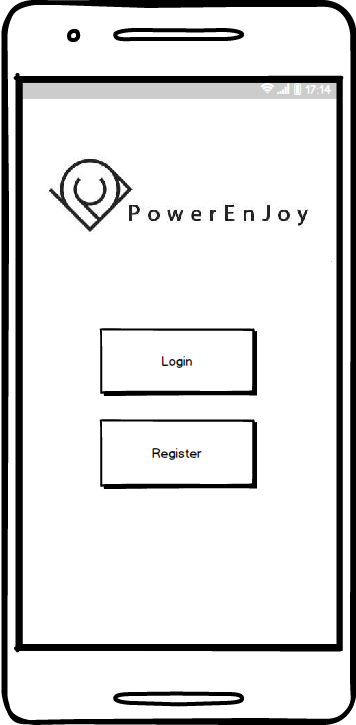
\includegraphics[scale=0.35]{img/mockups/App_guest.png}
			\caption{Guest view}
			\label{fig:subim1}
		\end{subfigure}
		\begin{subfigure}{0.5\textwidth}
			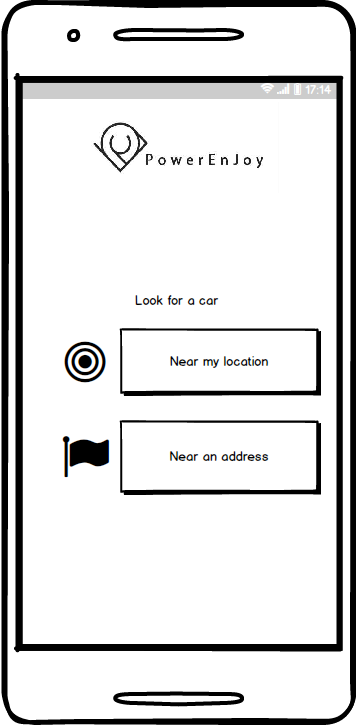
\includegraphics[scale=0.35]{img/mockups/App_user.png}
			\caption{User view}
			\label{fig:subim2}
		\end{subfigure}
 
		\caption{Mobile app: home page view}
		\label{fig:image1}
	\end{figure}
	
	\paragraph{} Figure 1 shows the first page that is shown when entering the app. Picture 1.a is the guest view, who has only the possibility of either logging in or registering in the system. Picture 1.b shows the user view. The user has more functionalities: they can look for cars in their vicinity or near an address, see and edit their profile, and changing settings (notification and sound settings). 
	
	\begin{figure}[h]
 
		\begin{subfigure}{0.3\paperwidth}
			\centering
			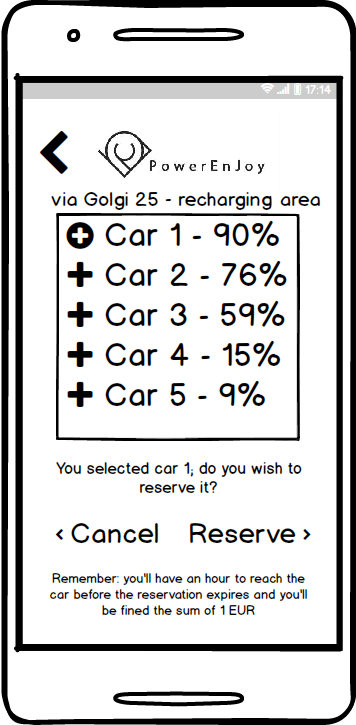
\includegraphics[scale=0.35]{img/mockups/User_reservation.png}
			\caption{View for the reservation}
			\label{fig:subim1}
		\end{subfigure}
		\begin{subfigure}{0.3\paperwidth}
			\centering
			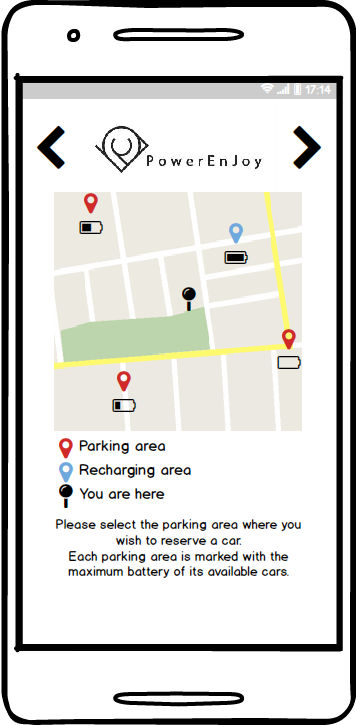
\includegraphics[scale=0.35]{img/mockups/User_parking_areas.png}
			\caption{View after having selected a parking area}
			\label{fig:subim2}
		\end{subfigure}
		\begin{subfigure}{0.3\paperwidth}
			\centering
			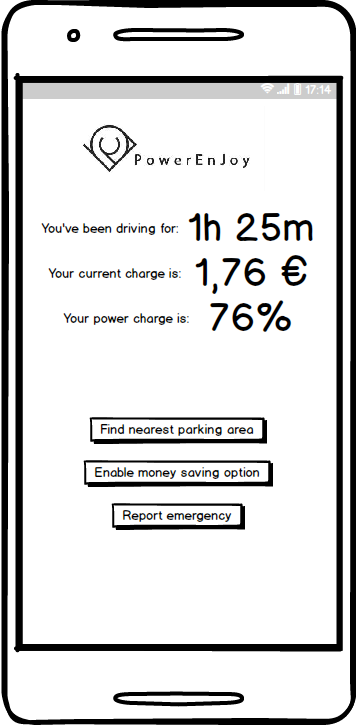
\includegraphics[scale=0.35]{img/mockups/User_driving.png}
			\caption{Display of the app while using a car}
			\label{fig:subim3}
		\end{subfigure}
 		
		
		\caption{Mobile app: main functionalities}
		\label{fig:image2}
	\end{figure}
	
	\paragraph{} Figure 2 shows the main functionalities of the \textit{PowerEnJoy}'s app: reserving a car (2.a and 2.b) and what you can do while using a car (2.c). 
	
	\begin{figure}
		\begin{subfigure}{1\textwidth}
			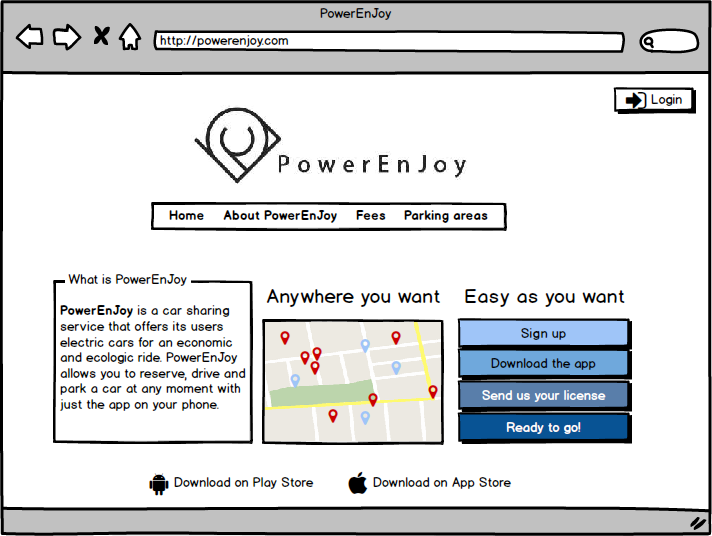
\includegraphics[scale=0.50]{img/mockups/Website.png}
			\caption{Website homepage}
			\label{fig:subim1}
		\end{subfigure}
		\begin{subfigure}{1\textwidth}
			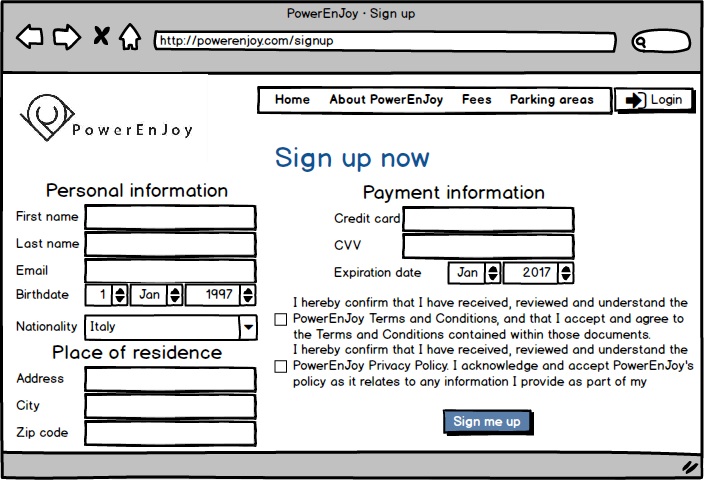
\includegraphics[scale=0.50]{img/mockups/Sign_up.png}
			\caption{Sign up on website}
			\label{fig:subim2}
		\end{subfigure}
		
		\caption{Website}
		\label{fig:image3}
	\end{figure}

	\paragraph{} Figure 3.a and 3.b shows, respectively, the website homepage from the standpoint of a guest and the sign up page. We haven't drawn the website mockup from the standpoint of a registered user since there are no more functionalities than those already present in the mobile app, as said above.

\FloatBarrier %to forbid images to enter the scenario chapter.

	\paragraph{Documentation}
	\paragraph{} In order to keep track of all phases of the development process and the overall structure of the system, the team will release the following documents:
		\begin{description}
			\item[RASD], Requirement Analysis and Specification Document, which provides a thorough description of the system, the requirements and the specification thanks to the use of UML models.
			\item[DD], Design Document, which contains a more in-depth description of the functionalities of the system.
			\item[ITPD], Integration Test Plan Document, which describes integration tests and the team's intended plan to accomplish them.
			\item[PP], Project Plan, which defines a planning for the development project.
			
			%do we need those last two??? 
		\end{description}